% Part-map for the Environment & Context Part (Ch1 "The shape of this book").
% Standalone TikZ; compiled by `book-scaffold build-figures` via pdflatex -> pdftocairo -> SVG.
% Environment (E1-E5) -> context-assembly boundary -> Context (C1-C3), with the C1->C2 arrow.
\documentclass[tikz,border=4mm]{standalone}
\usepackage{tikz}
\usetikzlibrary{positioning, arrows.meta, calc}

\begin{document}
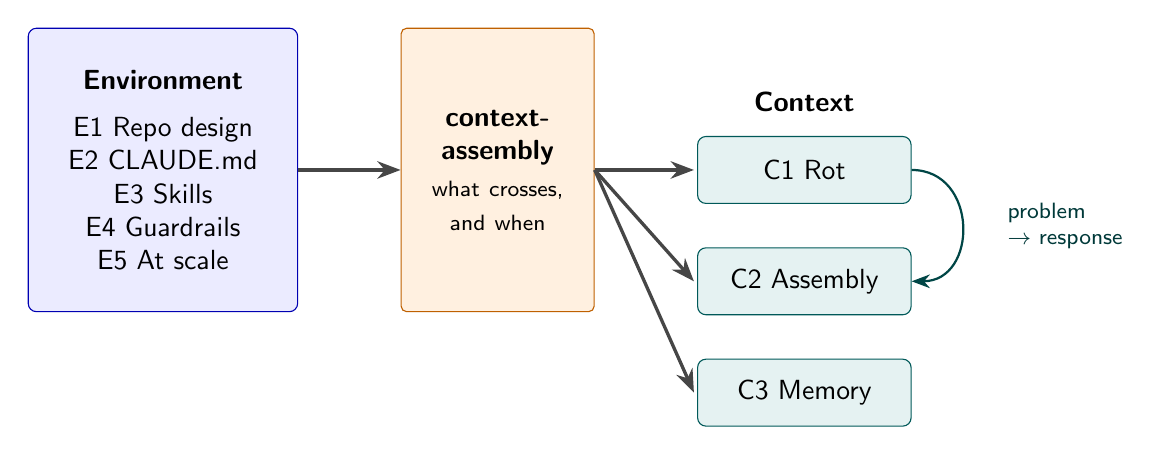
\begin{tikzpicture}[
  font=\sffamily,
  env/.style={draw=blue!70!black, fill=blue!8, rounded corners=3pt, align=center,
    text width=3.0cm, minimum height=3.6cm, inner sep=6pt},
  boundary/.style={draw=orange!75!black, fill=orange!12, rounded corners=2pt, align=center,
    text width=2.1cm, minimum height=3.6cm, inner sep=5pt},
  cbox/.style={draw=teal!70!black, fill=teal!10, rounded corners=3pt, align=center,
    text width=2.5cm, minimum height=0.85cm, inner sep=3pt},
  flow/.style={-Stealth, very thick, draw=gray!55!black},
  inner/.style={-Stealth, thick, draw=teal!55!black}
]

\node[env] (env) {{\bfseries Environment}\\[5pt]
  E1 Repo design\\
  E2 CLAUDE.md\\
  E3 Skills\\
  E4 Guardrails\\
  E5 At scale};

\node[boundary, right=1.3cm of env] (asm)
  {{\bfseries context-\\assembly}\\[4pt]\footnotesize what crosses,\\and when};

\node[cbox, right=1.3cm of asm] (c1) {C1 Rot};
\node[cbox, below=0.55cm of c1] (c2) {C2 Assembly};
\node[cbox, below=0.55cm of c2] (c3) {C3 Memory};
\node[font=\sffamily\bfseries, above=0.18cm of c1] {Context};

\draw[flow] (env) -- (asm);
\draw[flow] (asm.east) -- ($(c1.west)+(-0.04,0)$);
\draw[flow] (asm.east) -- ($(c2.west)+(-0.04,0)$);
\draw[flow] (asm.east) -- ($(c3.west)+(-0.04,0)$);

\draw[inner] (c1.east) .. controls +(0.85,0) and +(0.85,0) .. (c2.east)
  node[midway, right=0.45cm, font=\sffamily\footnotesize, align=left, text=teal!45!black]
  {problem\\$\to$ response};

\end{tikzpicture}
\end{document}
